\section{Problem B}
\textit{The achievable transmission rate R (bits/s) in a channel of bandwidth W (Hz) is related to the transmission power P (W) and noise power spectral density No (W/Hz) through the Shannon-Hartley formula:}
\begin{flalign}
 && R=& W\,\log_2\left(1+\frac{P}{W\,N_0}\right) &
\end{flalign}

\subsection{1)}
\textit{From the quantities entering the Shannon-Hartley formula, define Spectral Efficiency (SE), $\eta_{SE}$, in bps/Hz. Next, derive the trade-off between spectral efficiency and transmitted energy per bit, $E_b$. Plot the relation between SE and energy per bit, and conclude what is the best strategy in terms of minimising the energy consumption for a given fixed transmission rate R. As part of this, what is the minimum possible energy consumption per bit?}\\

By definition the Spectral Efficiency (SE) is given by the ratio between the bit Rate (R) and the Bandwidth (W). Using the Shannon formula the SE is:
\begin{flalign}
 && \eta _{SE}=& \frac{R}{W}= \,\log_2\left(1+\frac{P}{W\,N_0}\right) &
\end{flalign}
In order to get the trade-off between spectral efficiency and transmitted energy per bit the following steps are followed.\\
The energy per bit is given by:
\begin{flalign}
 && E_b=& \frac{P}{R} &
\end{flalign}
The power can be obtained from the equation 12.4 as:
\begin{flalign}
 && 2^{\eta _{SE}}=& \left(1+\frac{P}{W \cdot N_0}\right) &\\
 && P=& \left(2^{\eta _{SE}}-1\right)W\cdot N_0 & 
\end{flalign}
So, the equation 12.5 became as:
\begin{flalign}
&& E_b=& \dfrac{\left(2^{\eta _{SE}}-1\right)W\cdot N_0}{R} & \\
 &&=& \dfrac{\left(2^{\eta _{SE}}-1\right)\cdot N_0}{\eta _{SE}}
\end{flalign}
However, it is most common and interesting to plot the spectral efficiency in terms of $E_{b}/N_{o}$ (Energy per bit to noise power spectral density ratio). In the \figref{fig:Eb_SE} is plotted the relation between $\eta_{SE}$ and this parameter.

\begin{figure}[!h]
  \centering
  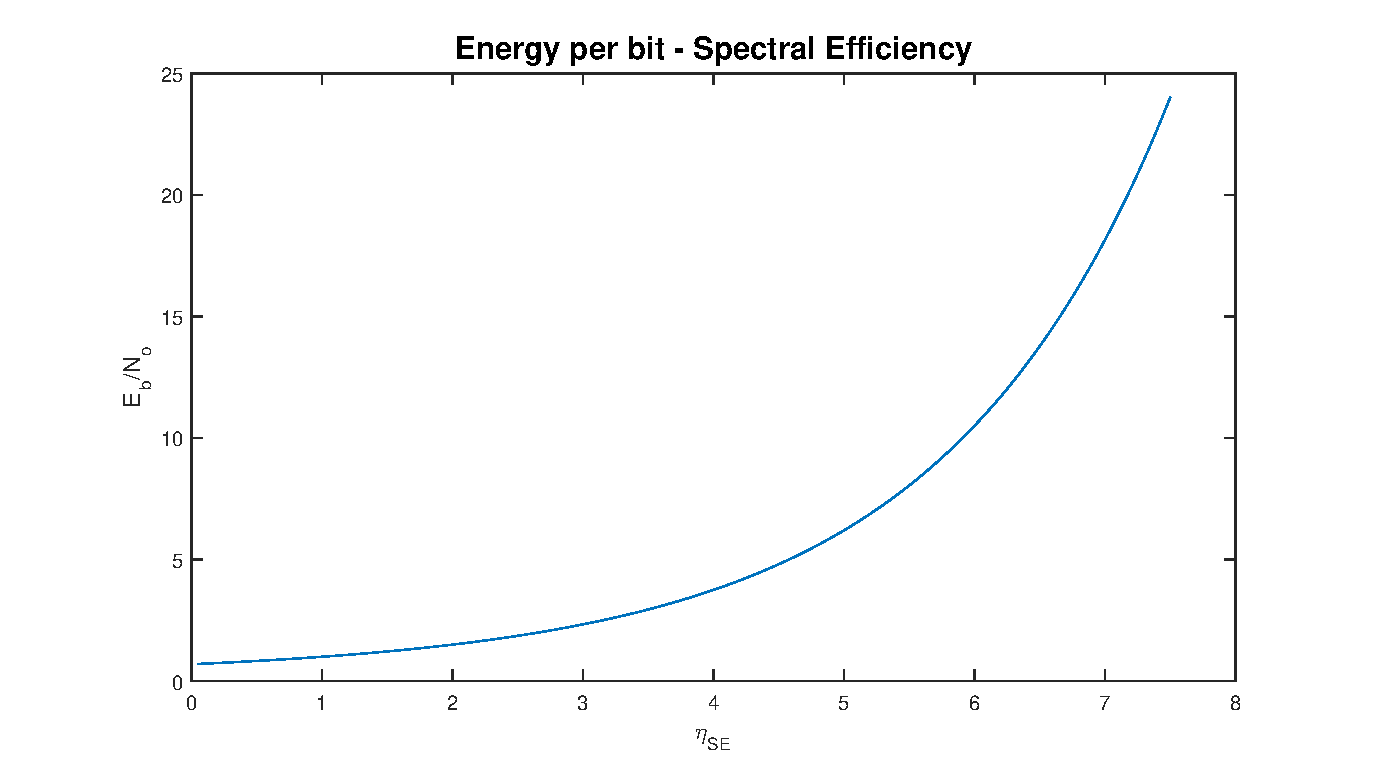
\includegraphics[width=14cm]{mm12_B1.eps}
  \caption{Relation between Energy per bit ($E_{b}$) and Spectral Efficiency ($\eta_{SE}$)}
  \label{fig:Eb_SE}
\end{figure}

\newpage

In order to minimize the energy consumption with a fixed data rate is necessary have a small spectral efficiency, which means have a wide bandwidth. As it can be seen in the figure, the minimum possible energy consumption per bit is about 0.7 for $\eta_{SE}$ equal to 0, which can be explained as:

\begin{flalign}
&& \lim_{\eta_{SE} \to 0} \frac{E_{b}}{N_{0}} = \lim_{\eta_{SE} \to 0} \dfrac{\left(2^{\eta _{SE}}-1\right)}{\eta _{SE}} =& \lim_{\eta_{SE} \to 0}  ln(2)\cdot 2^{\eta_{SE}} = 0.69 &
\end{flalign}



\subsection{2)}
\textit{Derive the trade-off between Spectral Efficiency (SE) and Energy Efficiency (EE) based on the Shannon-Hartley formula: Define EE, $\eta_{EE}$, in bits/Joule (naturally you would perhaps define Joule/bit, which however complicates things a bit), and then relate them via the formula.}\\

If we want to define the energy efficiency in bits/Joule we could obtained it by the inverse of the $E_{b}/N_{0}$ obtained in the previous section:

\begin{flalign}
&& \eta_{EE}=& \dfrac{N_{0}}{E_{b}} & \\
&&=&\dfrac{\eta _{SE}}{\left(2^{\eta _{SE}}-1\right)}
\end{flalign}

\textit{Sketch the relation in a graph and conclude whether it is possible to simultaneously maximise both quantities. As part of this, what happens to EE when SE approaches $0$ and $\infty$ (infinity), respectively?}\\

\begin{figure}[!h]
  \centering
  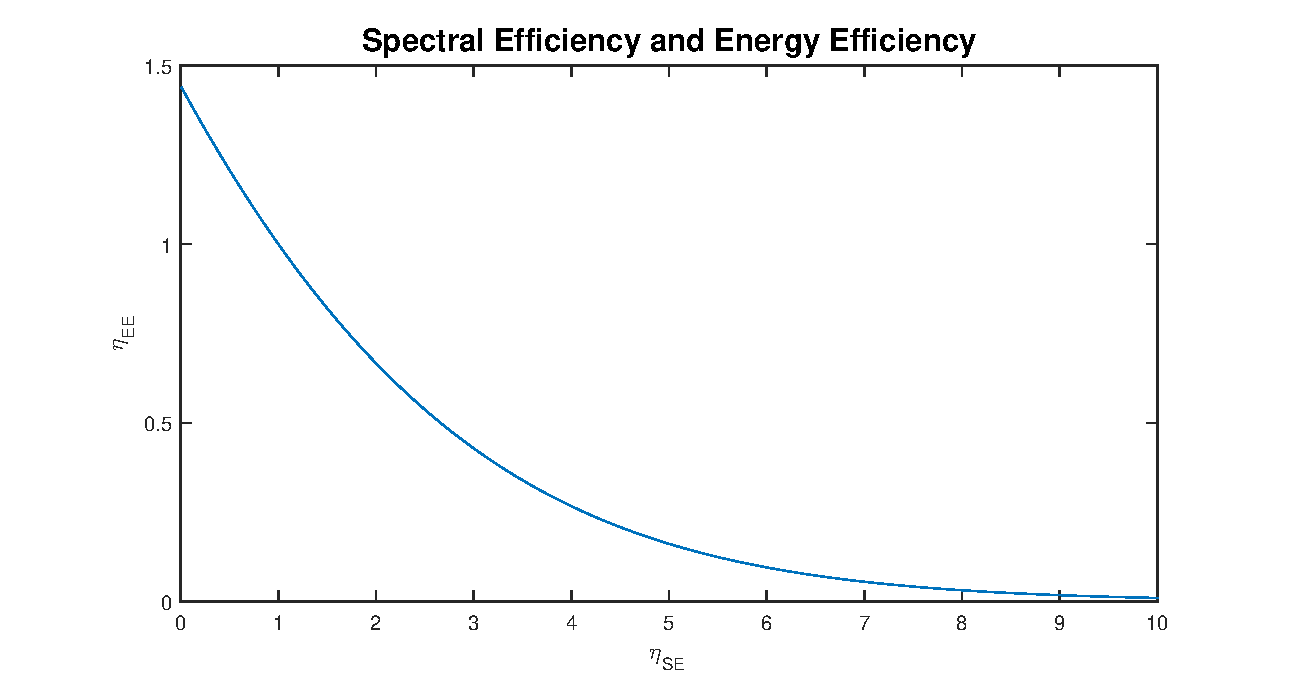
\includegraphics[width=14cm]{mm12_B2.eps}
  \caption{Relation between Energy Efficiency ($\eta_{SE}$) and Spectral Efficiency ($\eta_{SE}$)}
  \label{fig:EE_SE}
\end{figure}

From the plot we can conclude that the relation between $\eta_{SE}$ and $\eta_{EE}$ is inversely proportional, so is it not possible to maximise boh quantities at the same time. When the SE approaches to 0 the EE reaches its higher value (1.45) corresponded to the inverse of ln(2)). On the other hand, when SE approaches to $\infty$, the EE gets closer to 0.\\

\textit{The relation is a purely theoretical one which neglects several practical limitations, such as…?}\\

Some of the limitations are the bandwidth available or the maximum power that the transmitter can afford. Besides is convenient to remark that for the different modulations that can be used we would obtain different curves, but with similar patterns. 

